% Revised IEEE conference version (target: IEEE SANKALP 2027; verify the venue's author kit before submission).
% Build: see revised_manuscript/README.md. Figures are generated by statistical_reanalysis/05_figures.py.
\documentclass[conference]{IEEEtran}

\usepackage[T1]{fontenc}
\usepackage{cite}
\usepackage{amsmath}
\usepackage{amssymb}
\usepackage{booktabs}
\usepackage{graphicx}
\usepackage{array}
\usepackage{url}
\graphicspath{{figures/}}

\newcommand{\ppts}{\,pp}
\newcommand{\pfam}[1]{\textsf{#1}}

\begin{document}

\title{Does Perturbation Diversity Buy Robustness to Unseen Noise? A Family-Held-Out Study of Noisy LoRA Fine-Tuning}

\author{\IEEEauthorblockN{Soumya Ranjan Panda}
\IEEEauthorblockA{\textit{Independent Researcher}\\
soumyaranjanpanda.e@gmail.com}}

\maketitle

\begin{abstract}
Fine-tuning on deliberately perturbed inputs is a common way to make language models tolerate noisy text, and mixing several perturbation types is often assumed to prepare a model for perturbations it has never seen. Existing evidence confounds this assumption with the amount of corrupted data and with test-time exposure to the training perturbations. We test it in a controlled design whose protocol and decision rule were fixed before any test-set evaluation. Qwen2.5-0.5B-Instruct is fine-tuned with LoRA on BoolQ with half of the training questions corrupted, either by one perturbation family or by an equal mixture of three, and is evaluated on three other families that never occur in training. Over two folds of six families (54 training runs, three seeds), the mixture did not beat single-family training on held-out families: the pooled difference is $-0.14$ percentage points (pp), with an approximate 95\% interval of $[-0.77, +0.48]$ when both test-item and training-seed variability are included. The estimate is unchanged in direction after removing test items whose passage also occurs in training. Transfer between families was near zero or negative. The one family that caused a large drop, an irrelevant sentence appended to the question, lowered a clean-trained model's accuracy by 18.0\ppts{} and its rate of ``Yes'' answers by 25.9\ppts{}. Re-thresholding without labels recovered only 40 to 50\% of this loss, so the drop also reflects reduced discrimination. As few as 133 in-family training examples removed it. Code, data, run records, and per-item predictions are released.
\end{abstract}

\begin{IEEEkeywords}
robustness, noisy text, data augmentation, distribution shift, parameter-efficient fine-tuning, LoRA, negative results
\end{IEEEkeywords}

\section{Introduction}

\IEEEPARstart{L}{anguage} models deployed on real input meet typos, unusual formatting, dropped words, and irrelevant context. A standard remedy is to fine-tune on inputs that have been perturbed on purpose. Because no one can list every kind of noise in advance, practitioners often train on a \emph{mixture} of perturbation types, hoping that diversity induces an invariance that carries over to new noise. Mixed-type noisy instruction tuning has been reported to preserve or slightly improve accuracy under perturbed evaluation~\cite{alajrami2025noisy}, mixtures of synthetic noise improve translation of natural typos~\cite{karpukhin2019synthetic}, and in vision, diverse augmentation improves robustness to held-out corruptions~\cite{hendrycks2019benchmarking,hendrycks2020augmix}.

Two confounds make the text evidence hard to read. First, diversity usually varies together with \emph{volume}: a mixture condition often contains more corrupted examples than the single-type conditions it is compared with. Second, evaluation usually reuses the \emph{training} perturbation types, so a gain from mixing may only mean that the mixture covers more test types. Neither design shows whether diversity helps with noise the model has never seen. In vision, Mintun et al.~\cite{mintun2021interaction} found that augmentation gains shrink sharply on corruptions dissimilar to the augmentations, which makes the question worth testing for text rather than assuming.

We ask: \emph{at a fixed number of corrupted training examples, does a mixture of perturbation families generalise better to held-out families than a single family?} We fine-tune Qwen2.5-0.5B-Instruct~\cite{qwen2025qwen25} with LoRA~\cite{hu2022lora} on BoolQ~\cite{clark2019boolq}, holding data size, corrupted fraction (50\%), optimizer steps, and hyperparameters fixed. Six label-preserving families form two folds; each model trains on three families and is tested on the other three.

Our contributions are:
\begin{itemize}
  \item A family-held-out design that separates perturbation diversity from corruption volume and from test-time exposure, with clean, NEFTune~\cite{jain2024neftune}, and holdout-safe EDA~\cite{wei2019eda} baselines and a volume sweep.
  \item A pre-registered null result for this setting, with a post-hoc audit that separates test-item from training-seed uncertainty and checks sensitivity to train/test passage overlap. The audit shows that the original item-only interval understated uncertainty, while the null conclusion is stable.
  \item A family-by-family transfer matrix showing little transfer between families, and a descriptive account of how a distractor sentence degrades a small model: a shift towards ``No'' together with lower discrimination, both removed by a small amount of in-family data.
\end{itemize}
We do not claim that diversity never helps. Our results concern one 0.5B model, one task, synthetic question-level perturbations, and families that mostly leave little headroom.

\section{Related Work}
\label{sec:related}

\textit{Noisy fine-tuning.} Alajrami et al.~\cite{alajrami2025noisy} tune 7B to 72B models on instructions perturbed by six operations, sweeping the perturbed fraction at a fixed data size. Every perturbed run mixes all six types and evaluation applies the same types, so diversity is not separated from coverage. Li and Sen~\cite{li2026analyzing} train with one noise type at a time and evaluate on clean data only. Agrawal et al.~\cite{agrawal2025enhancing} train defences against perturbed instructions on mixtures that include the test attacks. Kumar et al.~\cite{kumar2020noisy} show that fine-tuning BERT on misspelled text degrades it. Karpukhin et al.~\cite{karpukhin2019synthetic} train on a mixture of synthetic character noise and test on natural typos, a held-out \emph{source} of noise but within the same broad family.

\textit{Robustness evaluation in NLP.} Belinkov and Bisk~\cite{belinkov2018synthetic} show that translation models break under synthetic and natural noise and that training on one noise kind does not reliably transfer to others. Rychalska et al.~\cite{rychalska2019wild} and Moradi and Samwald~\cite{moradi2021evaluating} measure sensitivity of pretrained models to families of character- and word-level corruptions, and Wang et al.~\cite{wang2022measure} survey robustness measurement and mitigation. Gokhale et al.~\cite{gokhale2022generalized} compare data modification methods for out-of-domain generalisation and adversarial robustness, and SSMBA~\cite{ng2020ssmba} uses augmentation for out-of-domain robustness. These works vary augmentation, but not perturbation diversity at fixed corruption volume with held-out families.

\textit{Transfer and held-out evaluation.} Hendrycks and Dietterich~\cite{hendrycks2019benchmarking} established evaluation on held-out image corruptions, and AugMix~\cite{hendrycks2020augmix} showed gains from diverse augmentation. Mintun et al.~\cite{mintun2021interaction} showed that such gains depend on augmentation-corruption similarity. Kang et al.~\cite{kang2019transfer} found that adversarial robustness often fails to transfer between perturbation types. Gulrajani and Lopez-Paz~\cite{gulrajani2021search} found, with leave-one-domain-out evaluation, that carefully tuned ERM matches domain generalisation methods: a negative result that our design mirrors at the level of perturbation families.

\textit{Distractors and answer bias.} Appending a distracting sentence is a classic stress test for reading comprehension~\cite{jia2017adversarial}, and large models are easily distracted by irrelevant context~\cite{shi2023distracted}. Zhao et al.~\cite{zhao2021calibrate} showed that language models carry input-dependent biases towards particular answers, which calibration can partly remove. We use this lens to read our distractor results.

\section{Research Questions}
\label{sec:rq}

\textbf{RQ1 (primary, pre-registered).} At 50\% corruption, is Mixed-3 more accurate on a fold's held-out families than the mean of the three single-family models? $H_1$: the difference is positive. The protocol declares an effect meaningful only if its 95\% interval excludes zero \emph{and} it exceeds the cross-seed SD of the effect. \textbf{RQ2 (secondary).} How does Mixed-3 compare with clean, NEFTune, and EDA training, and how much does robustness transfer between families? \textbf{RQ3 (descriptive).} Does raising the corrupted fraction change held-out accuracy? \textbf{RQ4 (exploratory, post hoc).} Why does the distractor family cause a large drop?

\section{Methodology}
\label{sec:method}

\subsection{Task, Data, and Model}
BoolQ~\cite{clark2019boolq} items are a passage, a yes/no question, and a label. We take the first 6{,}000 items of the BoolQ training split in dataset order and partition them into 4{,}000 training, 500 validation, 500 development, and 1{,}000 test items; 63.4\% of test labels are ``Yes''. No test question occurs in training, but BoolQ reuses Wikipedia passages: 136 test questions (121 of 969 distinct test passages) have a passage that also occurs verbatim in training, and 173 do when near-duplicates (5-gram Jaccard $\geq 0.5$) are counted. Section~\ref{sec:sens} reports results without these items. The model is Qwen2.5-0.5B-Instruct~\cite{qwen2025qwen25} with a fixed system prompt asking for ``Yes'' or ``No''.

\subsection{Perturbation Families}
Six label-preserving families perturb the \emph{question} only (Table~\ref{tab:families}). Perturbations are deterministic given a per-item seed; training and test perturbations use disjoint seed ranges, and all seven test versions contain the same 1{,}000 questions in the same order. The \pfam{distractor} family appends one of eight fluent, true, irrelevant sentences, without separating punctuation; training and test draw from the same eight sentences.

\begin{table}[t]
\centering
\caption{Perturbation Families and the Share of the 1{,}000 Test Questions Each Changes}
\label{tab:families}
\footnotesize
\setlength{\tabcolsep}{3pt}
\begin{tabular}{@{}l p{5.0cm} r@{}}
\toprule
Family & Operation & Changed \\
\midrule
\pfam{typo} & per letter, $p{=}0.05$: swap, keyboard-neighbour substitution, or deletion & 80.0\% \\
\pfam{formatting} & random case changes, punctuation removal/duplication, extra spaces & 98.1\% \\
\pfam{deletion} & drop each word with $p{=}0.15$ (keep $\geq 3$ words) & 77.5\% \\
\pfam{shuffle} & swap adjacent words with $p{=}0.2$ & 82.3\% \\
\pfam{distractor} & append one of 8 irrelevant true sentences & 100.0\% \\
\pfam{synonym} & replace content words, $p{=}0.3$, by a WordNet lemma~\cite{miller1995wordnet} & 79.7\% \\
\bottomrule
\end{tabular}
\end{table}

\subsection{Folds and Conditions}
Fold~A trains on \pfam{typo}, \pfam{formatting}, \pfam{deletion} and holds out \pfam{shuffle}, \pfam{distractor}, \pfam{synonym}; fold~B is the reverse. Every training set has exactly 4{,}000 examples. At 50\% corruption, items 1 to 2{,}000 are clean and items 2{,}001 to 4{,}000 are perturbed, so all conditions see the same questions. Per fold: three \emph{single-family} conditions; the primary \emph{Mixed-3} condition (667/667/666 examples of the three seen families); Mixed-3 at 10\%, 25\%, and 100\% corruption; and an EDA baseline~\cite{wei2019eda} restricted to operations that do not overlap the fold's held-out families. Shared across folds: \emph{clean} (no corruption) and \emph{NEFTune} (clean data, $\alpha{=}5$)~\cite{jain2024neftune}. The 18 conditions are trained with seeds 0, 1, 2, which set LoRA initialisation, dropout, and data order; with one untuned evaluation this gives 55 runs.

\subsection{Training and Evaluation}
All conditions share one configuration: LoRA $r{=}16$, $\alpha{=}32$, dropout 0.05 on all attention and MLP projections (8.8M trainable parameters); AdamW, learning rate $2{\times}10^{-4}$, 3\% warmup, cosine decay; 2 epochs at effective batch 16 (500 optimizer steps); loss on the answer and end-of-turn tokens only; 512-token limit enforced by truncating the passage (15 training items). Training used fp16 autocast on one NVIDIA T4 (mean 32\,min training and 10\,min evaluation per run). Each final model is evaluated once on all seven test versions. We compare the ``Yes'' and ``No'' next-token logits and predict ``Yes'' if $p(\text{Yes}) > 0.5$. In the released predictions, a median of 9 items (range 0 to 31) per run and test version have $p(\text{Yes})$ exactly 0.5 (fp16 logit ties), which this rule assigns to ``No''; Section~\ref{sec:sens} shows the conclusions do not depend on this.

\subsection{Statistical Analysis}
For fold $f$ the primary effect is
\begin{equation}
\Delta_f = \overline{\mathrm{acc}}_{U_f}(\text{Mixed-3}) - \tfrac{1}{3}\textstyle\sum_{k=1}^{3} \overline{\mathrm{acc}}_{U_f}(\text{single}_k),
\end{equation}
where $\overline{\mathrm{acc}}_{U_f}$ averages accuracy over the fold's held-out families $U_f$ and the three seeds, matched by seed. The pooled effect averages $\Delta_A$ and $\Delta_B$. The pre-registered interval is a 95\% percentile interval from 10{,}000 paired bootstrap resamples of test questions~\cite{efron1993bootstrap,koehn2004statistical}, applied jointly to every family, seed, and condition. It captures test-item uncertainty only.

\textit{Post-hoc additions} (not part of the protocol). (i) Because some test items share passages, we also resample passage clusters (966 clusters after merging identical and near-duplicate passages)~\cite{field2007bootstrapping}. (ii) Training randomness matters as much as test sampling~\cite{dodge2020fine,bouthillier2021accounting}, so we report per-seed effects, a $t$ interval over seeds, and an approximate combined interval $\Delta \pm 1.96\sqrt{\mathrm{SE}^2_{\text{items}} + \mathrm{SD}^2_{\text{seed}}/3}$, cross-checked with a two-stage bootstrap that resamples seeds within each condition and passage clusters jointly. With three seeds, every seed-level quantity is itself imprecise. (iii) We repeat the analysis without overlapping items, with alternative tie rules, and with a threshold-free score (probability assigned to the gold answer). (iv) For the 14 secondary contrasts we add Holm-adjusted bootstrap $p$-values, following common advice on significance testing in NLP~\cite{dror2018hitchhiker}.

\section{Results}
\label{sec:results}

All 55 runs completed, and the original analysis reproduces exactly from the released records. Three runs that were executed twice after cloud-session interruptions gave identical accuracies.

\subsection{RQ1: No Benefit From Diversity on Held-Out Families}
\label{sec:primary}

\begin{table*}[t]
\centering
\caption{Primary Effect $\Delta$ (Mixed-3 Minus Mean Single-Family Accuracy on the Fold's Held-Out Families, pp) Under the Pre-Registered Analysis and Post-Hoc Checks. Brackets: 95\% Intervals}
\label{tab:primary}
\footnotesize
\setlength{\tabcolsep}{8pt}
\begin{tabular}{@{}lccc@{}}
\toprule
 & Fold A & Fold B & Pooled \\
\midrule
Mixed-3 / mean single acc.\ (\%) & 69.06 / 69.76 & 77.18 / 76.76 & 73.12 / 73.26 \\
$\Delta$, item bootstrap (protocol) & $-0.71$ $[-1.38, -0.05]$ & $+0.42$ $[-0.24, +1.08]$ & $-0.14$ $[-0.59, +0.31]$ \\
Per-seed $\Delta$ (seeds 0, 1, 2) & $-1.17, -1.51, +0.56$ & $+0.88, +0.47, -0.08$ & $-0.14, -0.52, +0.24$ \\
Seed SD & 1.11 & 0.48 & 0.38 \\
Protocol verdict & not meaningful & null & null \\
\midrule
\multicolumn{4}{@{}l}{\emph{Post hoc (passage-cluster bootstrap unless stated)}} \\
Cluster bootstrap & $[-1.39, -0.03]$ & $[-0.25, +1.06]$ & $[-0.60, +0.30]$ \\
Items + seeds, approx. & $[-2.13, +0.72]$ & $[-0.43, +1.27]$ & $[-0.77, +0.48]$ \\
Two-stage bootstrap & $[-2.18, +0.76]$ & $[-0.62, +1.39]$ & $[-0.92, +0.62]$ \\
No verbatim overlap (864) & $-0.47$ $[-1.17, +0.21]$ & $+0.48$ $[-0.23, +1.18]$ & $+0.00$ $[-0.48, +0.47]$ \\
No near overlap (827) & $-0.53$ $[-1.24, +0.18]$ & $+0.46$ $[-0.30, +1.19]$ & $-0.04$ $[-0.52, +0.44]$ \\
Ties $=$ half credit & $-0.76$ $[-1.44, -0.09]$ & $+0.42$ $[-0.24, +1.05]$ & $-0.17$ $[-0.62, +0.27]$ \\
$p(\text{gold})$, threshold-free & $-0.85$ $[-1.24, -0.46]$ & $+0.33$ $[-0.09, +0.75]$ & $-0.26$ $[-0.53, +0.01]$ \\
\bottomrule
\end{tabular}
\end{table*}

\begin{figure}[t]
\centering
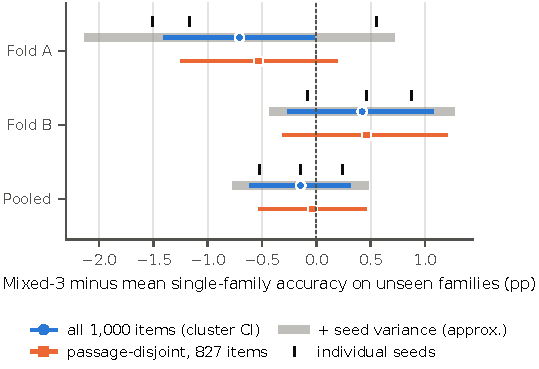
\includegraphics[width=\columnwidth]{fig_primary_effect.pdf}
\caption{Primary effect per fold. Blue: all items with passage-cluster 95\% CI; orange: items with no verbatim or near-duplicate passage in training; grey band: approximate interval including training-seed variance; ticks: individual seeds.}
\label{fig:primary}
\end{figure}

Mixing three families did not improve held-out accuracy in either fold (Table~\ref{tab:primary}, Fig.~\ref{fig:primary}). Fold~B's effect is small and its interval includes zero. Fold~A's point estimate is negative and its item-only interval just excludes zero, but the effect is smaller than its seed SD, so the pre-registered rule calls it not meaningful. The per-seed effects change sign in both folds, and dropping any one seed changes the fold~A estimate to between $-1.34$ and $-0.31$\ppts{}, so no single seed drives the pooled null.

\subsection{Sensitivity of the Primary Result}
\label{sec:sens}
Resampling passage clusters leaves the intervals essentially unchanged: 935 of 966 clusters are single questions. Adding training-seed variance widens the pooled interval from $[-0.59, +0.31]$ to about $[-0.77, +0.48]$ ($[-0.92, +0.62]$ by the two-stage bootstrap), so the data rule out a pooled benefit larger than roughly half a point, not 0.3\ppts{} as the item-only interval suggests. Removing overlapping items moves fold~A towards zero ($-0.47$\ppts{}) and makes the pooled estimate $0.00$; items with a training passage are 2 to 5\ppts{} easier for every condition. Tie handling changes estimates by at most 0.1\ppts{}. The threshold-free score agrees in direction: Mixed-3 assigns slightly less probability to the gold answer in fold~A. No setting produces evidence for $H_1$.

\subsection{RQ2: Baselines and Transfer}
\label{sec:secondary}
On fold~A's held-out families, Mixed-3 was less accurate than clean training ($-2.29$\ppts{}, cluster CI $[-3.12, -1.46]$), NEFTune ($-2.06$, $[-2.95, -1.17]$), and EDA ($-1.24$, $[-2.10, -0.42]$). All three survive the combined item-and-seed interval and Holm correction (adjusted $p \leq 0.044$) and the no-overlap subset. On clean test data, Mixed-3 and clean training are indistinguishable ($-0.57$, $[-1.67, +0.56]$). In fold~B, Mixed-3 was indistinguishable from every baseline on held-out families. Mixed-3 beat the mean single-family model on fold~B's \emph{seen} families ($+4.51$\ppts{}), but this follows from the design: only one of the three single-family models saw \pfam{distractor}, the one family where training matters.

\begin{figure}[t]
\centering
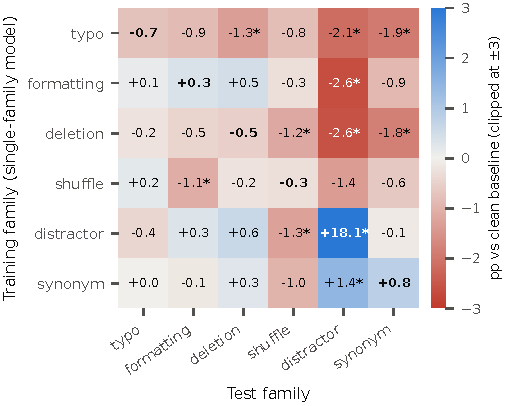
\includegraphics[width=0.94\columnwidth]{fig_transfer_matrix.pdf}
\caption{Accuracy of each single-family model minus the clean baseline (pp, mean of 3 seeds). Bold: tested on the training family. *: passage-cluster 95\% CI excludes 0 (test-item uncertainty only). Colour clipped at $\pm$3\ppts{}.}
\label{fig:transfer}
\end{figure}

Fig.~\ref{fig:transfer} explains both results. Five families cost a clean-trained model at most 3.7\ppts{} relative to its 78.8\% clean accuracy, and training on a family changes accuracy on that same family by less than 1\ppts{}, leaving little room for transfer. \pfam{Distractor} is the exception: training on it recovers $+18.1$\ppts{} (CI $[+15.0, +21.2]$), while off-diagonal entries in its column range from $-2.6$ to $+1.4$\ppts{}. The fold~A training families (\pfam{typo}, \pfam{formatting}, \pfam{deletion}) each \emph{lower} \pfam{distractor} accuracy by 2.1 to 2.6\ppts{}, which accounts for part of fold~A's deficit against clean training.

\textit{Held-out versus in-family evaluation.} For five families, a Mixed-3 model's accuracy differs by less than 3\ppts{} between the fold where the family was trained on and the fold where it was held out. For \pfam{distractor} the gap is 21.6\ppts{} (79.1\% vs.\ 57.5\%). Evaluating only on training families would have hidden this weakness, but the hidden weakness concerns one family, not noise in general.

\subsection{RQ3: Corruption Volume}
Raising Mixed-3's corrupted fraction from 10\% to 100\% did not raise held-out accuracy. Fold~B stayed within 0.7\ppts{} of clean training at every fraction (76.5 to 77.2\%). In fold~A, accuracy at 50\% and 100\% was about 2\ppts{} below clean training (69.1 and 69.2\% vs.\ 71.3\%). The sweep was specified as descriptive and is not tested.

\subsection{RQ4: Anatomy of the Distractor Drop (Exploratory)}
\label{sec:distractor}

\begin{figure*}[t]
\centering
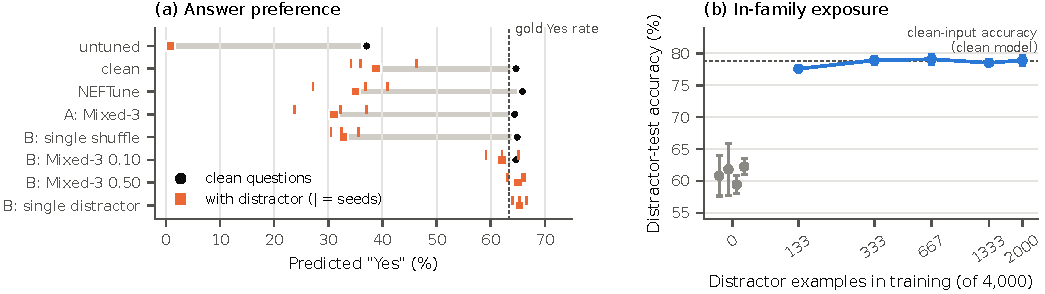
\includegraphics[width=\textwidth]{fig_distractor_bias.pdf}
\caption{(a) Share of ``Yes'' predictions on clean questions and on the same questions with a distractor (mean of 3 seeds; ticks: seeds). (b) Distractor-test accuracy against the number of distractor examples among the 4{,}000 training examples (fold~B conditions; grey points at 0: clean, EDA, single \pfam{shuffle}, single \pfam{synonym}). Error bars: $\pm$1 SD over seeds.}
\label{fig:distractor}
\end{figure*}

The appended sentence pushes models towards ``No'' (Fig.~\ref{fig:distractor}a). The untuned model answers ``Yes'' to 0.8\% of distractor questions (37.1\% on clean questions). For the clean-trained model the ``Yes'' rate falls by 25.9\ppts{} (CI $[-28.7, -23.0]$) and accuracy by 18.0\ppts{}; of the items it loses, 91\% are Yes-to-No flips. Across the 39 trained runs without distractor data, the per-run shift in ``Yes'' rate and the accuracy drop correlate at $r = 0.81$. The size of the shift also explains the large seed SD on this family.

The shift is not the whole story. Discrimination drops as well: the clean model's AUC falls from 0.852 to 0.728, and from 0.852 to 0.747 when computed within groups that share the same distractor sentence. Moving the decision threshold so that the distractor ``Yes'' rate matches the same model's clean rate, which uses no labels, raises accuracy from 60.8\% to 68.1\%, 41\% of the loss (70.1\%, or 52\%, with one threshold per sentence). The effect also depends strongly on the sentence: for the clean model, one sentence does not lower the ``Yes'' rate ($+6.1$\ppts{}) while two lower it by more than 50\ppts{}, with 96 to 145 test items per sentence.

Small amounts of in-family data remove both effects (Fig.~\ref{fig:distractor}b). Fold~B's Mixed-3 at 10\% corruption, with 133 distractor examples, reaches 77.6\% on distractor questions with a ``Yes'' rate of 62.1\%; with 333 or more examples, accuracy matches the clean-input level and AUC returns to 0.84 to 0.85. Because training and test share the eight sentences, part of this gain may be familiarity with the sentences rather than a general skill.

\section{Discussion}
\label{sec:discussion}

A mixture can only beat its components on held-out families if training on some families confers robustness to others. Fig.~\ref{fig:transfer} shows almost none, so diversity had nothing to combine. This matches the vision finding that augmentation helps mainly on similar corruptions~\cite{mintun2021interaction,kang2019transfer}, and it suggests that ``diverse noise as insurance'' should be measured rather than assumed for small models. Diversity was not harmful on the families it covered: fold~B's Mixed-3 was as robust to \pfam{distractor} as the dedicated model with a third of the examples. Mixing is a reasonable way to cover \emph{known} perturbations; in our setting it did not reach unknown ones.

Perturbed training was also not free. In fold~A, surface and deletion noise left models less robust to held-out perturbations than clean training, mostly through a stronger ``No'' shift on distractor questions. We have no mechanism for this, and fold~B shows no such cost. For robustness evaluation, the distractor results suggest reporting answer-rate statistics and threshold-free discrimination next to accuracy, since an accuracy drop can combine a prior shift that calibration can address~\cite{zhao2021calibrate} with a genuine loss of information.

\section{Threats to Validity and Limitations}
\label{sec:limitations}

\textit{External validity.} One 0.5B model, one binary reading task, three seeds, and synthetic perturbations of the question only. The optional 1.5B check in the protocol was not run. Larger models may transfer robustness more readily~\cite{alajrami2025noisy}.

\textit{Power and headroom.} Five of six families cost the clean model at most 3.7\ppts{}, which bounds any diversity effect on them. The folds are asymmetric: fold~A's held-out set contains the hard, high-variance \pfam{distractor} family, while fold~B's held-out families are nearly solved by clean training.

\textit{Construct validity.} WordNet substitution is only approximately meaning-preserving. The distractor is appended without punctuation and comes from eight shared sentences, so its effects may be specific to this construction.

\textit{Statistical conclusion validity.} Three seeds give imprecise estimates of training variance; the combined intervals are approximations. Secondary contrasts were not corrected in the protocol, and the overlap, tie, cluster, and distractor analyses were all added after the results were known. Runs used two PyTorch versions (2.11 and 2.14, aligned mostly with seed index rather than condition).

\section{Conclusion}
\label{sec:conclusion}

At a fixed corruption volume, fine-tuning Qwen2.5-0.5B-Instruct on a mixture of three perturbation families did not make it more robust to held-out families than training on one family, and neither did more corrupted data. The null survives passage-overlap removal and explicit accounting for seed variance, with a pooled benefit larger than about half a point ruled out. Robustness was family-specific: the one perturbation that caused a large drop combined an answer shift with lost discrimination, and only data containing it fixed the problem. Natural next steps are larger models, more tasks, and perturbation families with more headroom for transfer.

\section*{Code and Data Availability}
Code, data, SHA-256 manifests, per-run configurations, training logs, and per-item predictions for all 55 runs are at \url{https://github.com/SoumyaranjanPanda01/noise-diversity-research}. The protocol, deviations, and every post-hoc analysis in this paper (folder \texttt{statistical\_reanalysis/}) are included and run on a CPU.

\begin{thebibliography}{99}

\bibitem{alajrami2025noisy}
A.~Alajrami, X.~Tan, and N.~Aletras, ``Fine-tuning on noisy instructions: Effects on generalization and performance,'' in \emph{Proc. IJCNLP-AACL}, 2025, arXiv:2510.03528.

\bibitem{karpukhin2019synthetic}
V.~Karpukhin, O.~Levy, J.~Eisenstein, and M.~Ghazvininejad, ``Training on synthetic noise improves robustness to natural noise in machine translation,'' in \emph{Proc. 5th Workshop Noisy User-Generated Text (W-NUT)}, 2019, pp.~42--47.

\bibitem{hendrycks2019benchmarking}
D.~Hendrycks and T.~Dietterich, ``Benchmarking neural network robustness to common corruptions and perturbations,'' in \emph{Proc. ICLR}, 2019.

\bibitem{hendrycks2020augmix}
D.~Hendrycks, N.~Mu, E.~D. Cubuk, B.~Zoph, J.~Gilmer, and B.~Lakshminarayanan, ``{AugMix}: A simple data processing method to improve robustness and uncertainty,'' in \emph{Proc. ICLR}, 2020.

\bibitem{mintun2021interaction}
E.~Mintun, A.~Kirillov, and S.~Xie, ``On interaction between augmentations and corruptions in natural corruption robustness,'' in \emph{Proc. NeurIPS}, 2021.

\bibitem{qwen2025qwen25}
Qwen Team, ``{Qwen2.5} technical report,'' 2025, arXiv:2412.15115.

\bibitem{hu2022lora}
E.~J. Hu \emph{et al.}, ``{LoRA}: Low-rank adaptation of large language models,'' in \emph{Proc. ICLR}, 2022.

\bibitem{clark2019boolq}
C.~Clark, K.~Lee, M.-W. Chang, T.~Kwiatkowski, M.~Collins, and K.~Toutanova, ``{BoolQ}: Exploring the surprising difficulty of natural yes/no questions,'' in \emph{Proc. NAACL-HLT}, 2019, pp.~2924--2936.

\bibitem{jain2024neftune}
N.~Jain \emph{et al.}, ``{NEFTune}: Noisy embeddings improve instruction finetuning,'' in \emph{Proc. ICLR}, 2024.

\bibitem{wei2019eda}
J.~Wei and K.~Zou, ``{EDA}: Easy data augmentation techniques for boosting performance on text classification tasks,'' in \emph{Proc. EMNLP-IJCNLP}, 2019, pp.~6382--6388.

\bibitem{li2026analyzing}
L.~Li and P.~Sen, ``Analyzing the effect of noise in {LLM} fine-tuning,'' 2026, arXiv:2604.12469.

\bibitem{agrawal2025enhancing}
A.~Agrawal, L.~Alazraki, S.~Honarvar, and M.~Rei, ``Enhancing {LLM} robustness to perturbed instructions: An empirical study,'' in \emph{Proc. ICLR Workshop Building Trust in Lang. Models and Appl.}, 2025, arXiv:2504.02733.

\bibitem{kumar2020noisy}
A.~Kumar, P.~Makhija, and A.~Gupta, ``Noisy text data: {Achilles'} heel of {BERT},'' in \emph{Proc. 6th Workshop Noisy User-Generated Text (W-NUT)}, 2020, pp.~16--21.

\bibitem{belinkov2018synthetic}
Y.~Belinkov and Y.~Bisk, ``Synthetic and natural noise both break neural machine translation,'' in \emph{Proc. ICLR}, 2018.

\bibitem{rychalska2019wild}
B.~Rychalska, D.~Basaj, A.~Gosiewska, and P.~Biecek, ``Models in the wild: On corruption robustness of neural {NLP} systems,'' in \emph{Proc. ICONIP}, ser. LNCS, vol. 11955, 2019, pp.~235--247.

\bibitem{moradi2021evaluating}
M.~Moradi and M.~Samwald, ``Evaluating the robustness of neural language models to input perturbations,'' in \emph{Proc. EMNLP}, 2021, pp.~1558--1570.

\bibitem{wang2022measure}
X.~Wang, H.~Wang, and D.~Yang, ``Measure and improve robustness in {NLP} models: A survey,'' in \emph{Proc. NAACL}, 2022, pp.~4569--4586.

\bibitem{gokhale2022generalized}
T.~Gokhale, S.~Mishra, M.~Luo, B.~S. Sachdeva, and C.~Baral, ``Generalized but not robust? {C}omparing the effects of data modification methods on out-of-domain generalization and adversarial robustness,'' in \emph{Findings ACL}, 2022, pp.~2705--2718.

\bibitem{ng2020ssmba}
N.~Ng, K.~Cho, and M.~Ghassemi, ``{SSMBA}: Self-supervised manifold based data augmentation for improving out-of-domain robustness,'' in \emph{Proc. EMNLP}, 2020, pp.~1268--1283.

\bibitem{kang2019transfer}
D.~Kang, Y.~Sun, T.~Brown, D.~Hendrycks, and J.~Steinhardt, ``Transfer of adversarial robustness between perturbation types,'' 2019, arXiv:1905.01034.

\bibitem{gulrajani2021search}
I.~Gulrajani and D.~Lopez-Paz, ``In search of lost domain generalization,'' in \emph{Proc. ICLR}, 2021.

\bibitem{jia2017adversarial}
R.~Jia and P.~Liang, ``Adversarial examples for evaluating reading comprehension systems,'' in \emph{Proc. EMNLP}, 2017, pp.~2021--2031.

\bibitem{shi2023distracted}
F.~Shi \emph{et al.}, ``Large language models can be easily distracted by irrelevant context,'' in \emph{Proc. ICML}, PMLR vol. 202, 2023, pp.~31210--31227.

\bibitem{zhao2021calibrate}
T.~Z. Zhao, E.~Wallace, S.~Feng, D.~Klein, and S.~Singh, ``Calibrate before use: Improving few-shot performance of language models,'' in \emph{Proc. ICML}, PMLR vol. 139, 2021, pp.~12697--12706.

\bibitem{miller1995wordnet}
G.~A. Miller, ``{WordNet}: A lexical database for {English},'' \emph{Commun. ACM}, vol.~38, no.~11, pp.~39--41, 1995.

\bibitem{efron1993bootstrap}
B.~Efron and R.~J. Tibshirani, \emph{An Introduction to the Bootstrap}. New York, NY, USA: Chapman \& Hall, 1993.

\bibitem{koehn2004statistical}
P.~Koehn, ``Statistical significance tests for machine translation evaluation,'' in \emph{Proc. EMNLP}, 2004, pp.~388--395.

\bibitem{field2007bootstrapping}
C.~A. Field and A.~H. Welsh, ``Bootstrapping clustered data,'' \emph{J. Roy. Statist. Soc. B}, vol.~69, no.~3, pp.~369--390, 2007.

\bibitem{dodge2020fine}
J.~Dodge, G.~Ilharco, R.~Schwartz, A.~Farhadi, H.~Hajishirzi, and N.~Smith, ``Fine-tuning pretrained language models: Weight initializations, data orders, and early stopping,'' 2020, arXiv:2002.06305.

\bibitem{bouthillier2021accounting}
X.~Bouthillier \emph{et al.}, ``Accounting for variance in machine learning benchmarks,'' in \emph{Proc. MLSys}, 2021.

\bibitem{dror2018hitchhiker}
R.~Dror, G.~Baumer, S.~Shlomov, and R.~Reichart, ``The hitchhiker's guide to testing statistical significance in natural language processing,'' in \emph{Proc. ACL}, 2018, pp.~1383--1392.

\end{thebibliography}

\end{document}
